\documentclass[12pt]{beamer}
\usepackage[utf8]{inputenc}
\usepackage[spanish]{babel}
%\usepackage{graphicx}
%\usepackage[pdftex]{hyperref}
\usepackage{listings}
\usepackage{eurofont}
\usepackage{lmodern}

%\usetheme{Warsaw}
%\mode<presentation>
%{ \usetheme{boxes} }


% Comment the next line to create a printable version
\beamerdefaultoverlayspecification{<+->}
\setbeamercovered{transparent}
\usepackage{keynote-gradient}

\title{Programación mediante tarjetas gráficas}
\subtitle{Mejora de una aplicación distribuida}
\author{Samuel Rodríguez Sevilla\\Tutor: José María Sierra Cámara}


\begin{document}


\frame{\titlepage}

%\begin{frame}
%	\begin{center}
%		\Huge iCrack
%	\end{center}
%\end{frame}


\begin{frame}{Contenidos}
	\tableofcontents[pausesections]
\end{frame}

\section{Introducción}
\begin{frame}{Introducción}
	\begin{itemize}
		\item La seguridad es muy importante actualmente
		\item Hay muchos factores que afectan a la seguridad
		\begin{itemize}
			\item Fallos de programación de las aplicaciones
			\item Mala configuración de los sistemas
			\item Factores humanos
		\end{itemize}
	\end{itemize}
\end{frame}

\begin{frame}{Introducción}
	El factor humano es probablemente el que más afecta a la seguridad ya que no hay una verdadera concienciación sobre los peligros que entraña revelar claves.

\end{frame}

\begin{frame}{Introducción}
	Por esto es importente
	\pause
	\begin{itemize}
		\item Disponer de buenas políticas para las contraseñas
		\item Utilizar herramientas para evaluar la calidad de los algoritmos utilizados
	\end{itemize}
\end{frame}

\subsection{Objetivos}
\begin{frame}{Objetivos}
	\begin{center}
		Obtener una herramienta capaz de evaluar algoritmos de seguridad y contraseñas haciendo uso de tarjetas gráficas.
	\end{center}
\end{frame}

\begin{frame}{Objetivos}
	\begin{itemize}
		\item Sencilla de utilizar
		\item Ampliable con nuevos algoritmos
		\item Distribuida
		\item Libre
	\end{itemize}
\end{frame}

\subsection{Uso de tarjetas gráficas}
\begin{frame}{Uso de tarjetas gráficas}
	\begin{center}
		Su velocidad ha crecido mucho~\cite{nvidia:cuda_c_programming_guide} y han añadido nuevas características que las hacen muy atractivas para todo tipo de tareas.
	\end{center}
\end{frame}


\lstset{emph={int,float,void}, emphstyle=\color{blue},
emph={[2]__global__,__device__,__kernel__,threadIdx},emphstyle={[2]\color{green}}}
\defverbatim[colored]\testcode{%
\begin{lstlisting}[frame=single]
__global__ void vector_add(
  float *v1, float *v2, float *r)
{
  int p = threadIdx.x;
  r[p] = v1[p] + v2[p];
}
\end{lstlisting}}
\begin{frame}{Uso de tarjetas gráficas}
	Entre sus principales características destacan:
	\pause

	\begin{itemize}
		\item Una gran velocidad realizando operaciones aritméticas
		\only<2>{
			\begin{figure}
				\centering
				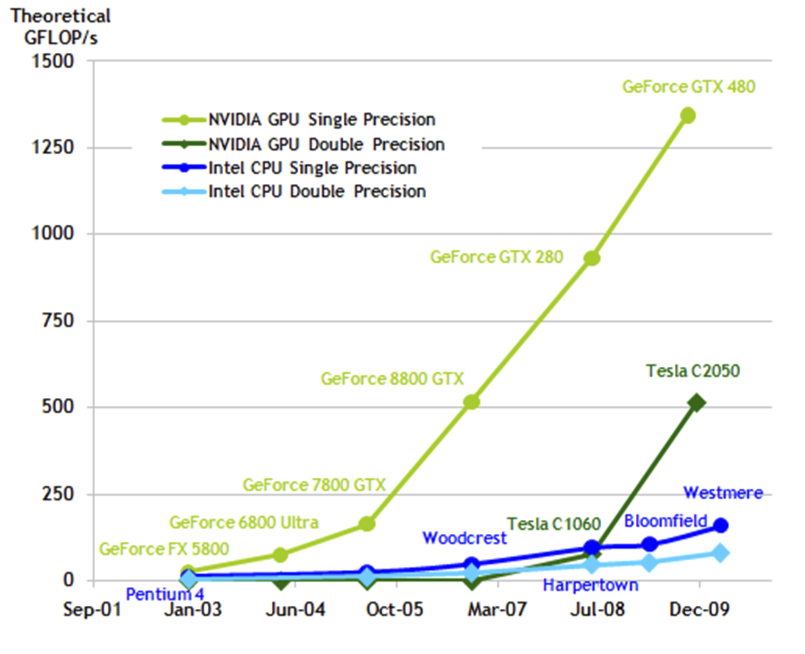
\includegraphics[width=0.5\textwidth]{images/evolucion-gpu.png}
				\caption{Incremento de los FLOPS en CPU y GPU (fuente~\cite{nvidia:cuda_c_programming_guide})}
			\end{figure}
		}
			
		\item Gran capacidad para el paralelismo
			\only<3>{
				\begin{figure}
					\centering
					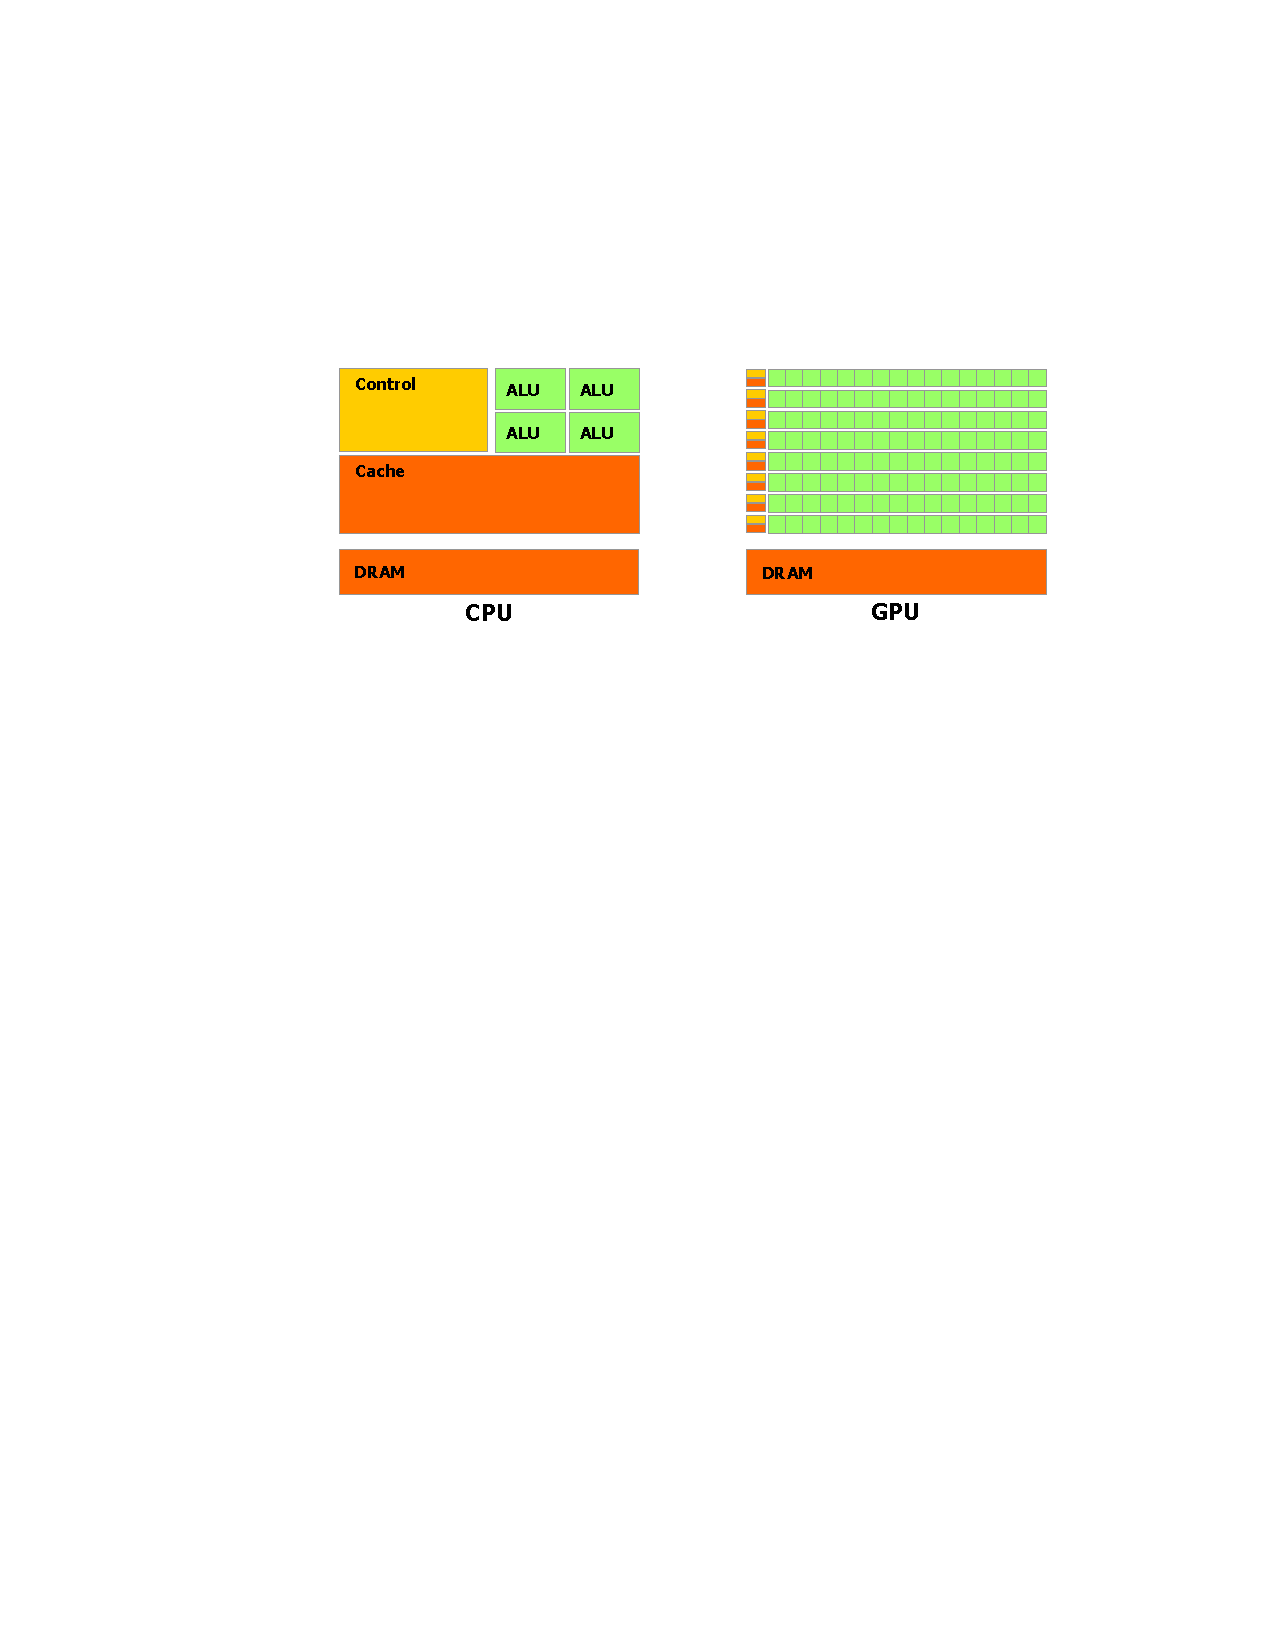
\includegraphics[width=0.7\textwidth]{images/cpuvsgpu.pdf}
					\caption{Comparación interna CPU y GPU (fuente~\cite{nvidia:cuda_c_programming_guide})}			
				\end{figure}
			}
			
		\item Son fáciles de programar
			\only<4>{
				\testcode
			}
	\end{itemize}
\end{frame}

\section{DHC}
\begin{frame}{DHC}
	Se tomó como base de las modificaciones por varios motivos:
	\pause
	\begin{itemize}
		\item Es software libre
		\item Cumplía casi todos los requisitos
		\item Es la única herramienta gratuita de este tipo
	\end{itemize}
\end{frame}

\begin{frame}{DHC}
	\begin{center}
		Pero a pesar de todo, también tiene algunas carencias...		
	\end{center}
\end{frame}


\section{Mejoras introducidas}

\subsection{Mejora de la escalabilidad}
\begin{frame}{Mejora de la escalabilidad}
	\begin{center}
		DHC pierde mucha velocidad debido a las latencias de red.
		% Esto se constata cuando se tiene una instalación...
	\end{center}
\end{frame}


\subsection{Sistema de algoritmos}
\begin{frame}{Sistema de algoritmos}
	\begin{center}
		Sustituye el código estático de DHC y facilita la carga de nuevos algoritmos sin tener que hacer modificaciones sobre una gran cantidad de códigos.
	\end{center}
\end{frame}

\subsection{Sistema de ejecución}
\begin{frame}{Sistema de ejecución}
	\begin{center}
		Homogeniza el modo en el que se ejecutan los algoritmos.
	\end{center}
\end{frame}

\subsection{Carga de plugins}
\begin{frame}{Carga de plugins}
	\begin{center}
		Facilita la creación de algoritmos sin tener que cambiar una sola línea de código del agente.
	\end{center}
\end{frame}

\subsection{Nuevo controlador}
\begin{frame}{Nuevo controlador}

\end{frame}



\section{Presupuesto}
\begin{frame}{Presupuesto}
	\begin{center}
		43.785,30\euro
	\end{center}
\end{frame}


\section{Conclusiones y trabajos futuros}
\subsection{Conclusiones}
\begin{frame}{Conclusiones}
\end{frame}

\subsection{Trabajos futuros}
\begin{frame}{Trabajos futuros}
\end{frame}

\begin{frame}
	\begin{center}
		\Huge Fin
	\end{center}
\end{frame}

\section{Bibliografía}
\begin{frame}[allowframebreaks]{Bibliografía}
	\bibliographystyle{alpha}
	\bibliography{bibliografia}
\end{frame}
\end{document}
